\section{Конструкторская часть}

\subsection*{Разработка алгоритмов}
\addcontentsline{toc}{subsection}{Разработка алгоритмов}
На рисунке \ref{img:brute} приведена схема алгоритма решения задачи коммивояжера полным перебором. Схемы муравьиного алгоритма приведена на рисунке \ref{img:ant}, вспомогательные функции данного алгоритма показаны на рисунках \ref{img:probability}-\ref{img:update}.

\begin{figure}[hbtp]
	\centering
	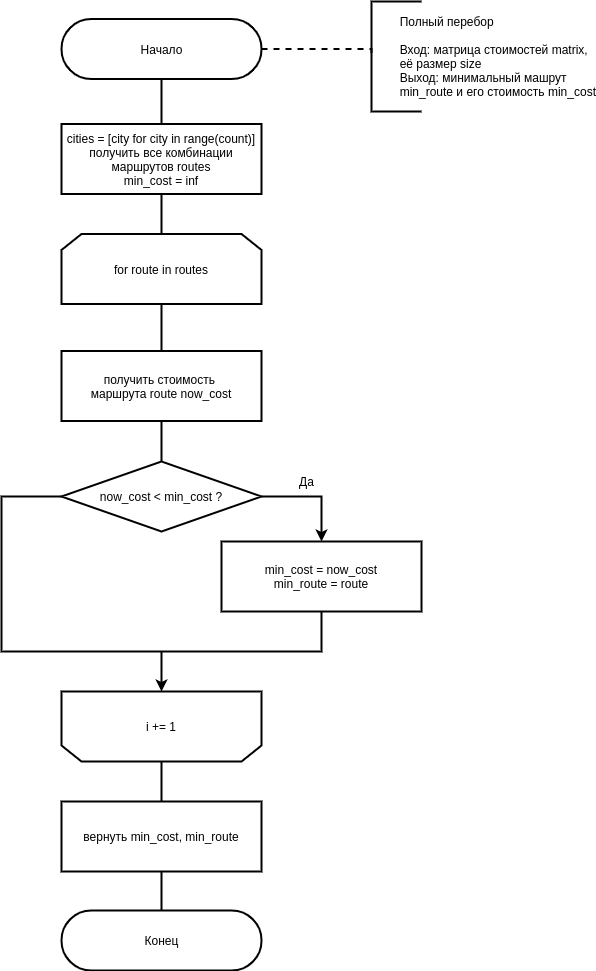
\includegraphics[scale=0.5]{images/brute.png}
	\caption{Полный перебор}
	\label{img:brute}
\end{figure}

\begin{figure}[!h]
	\centering
	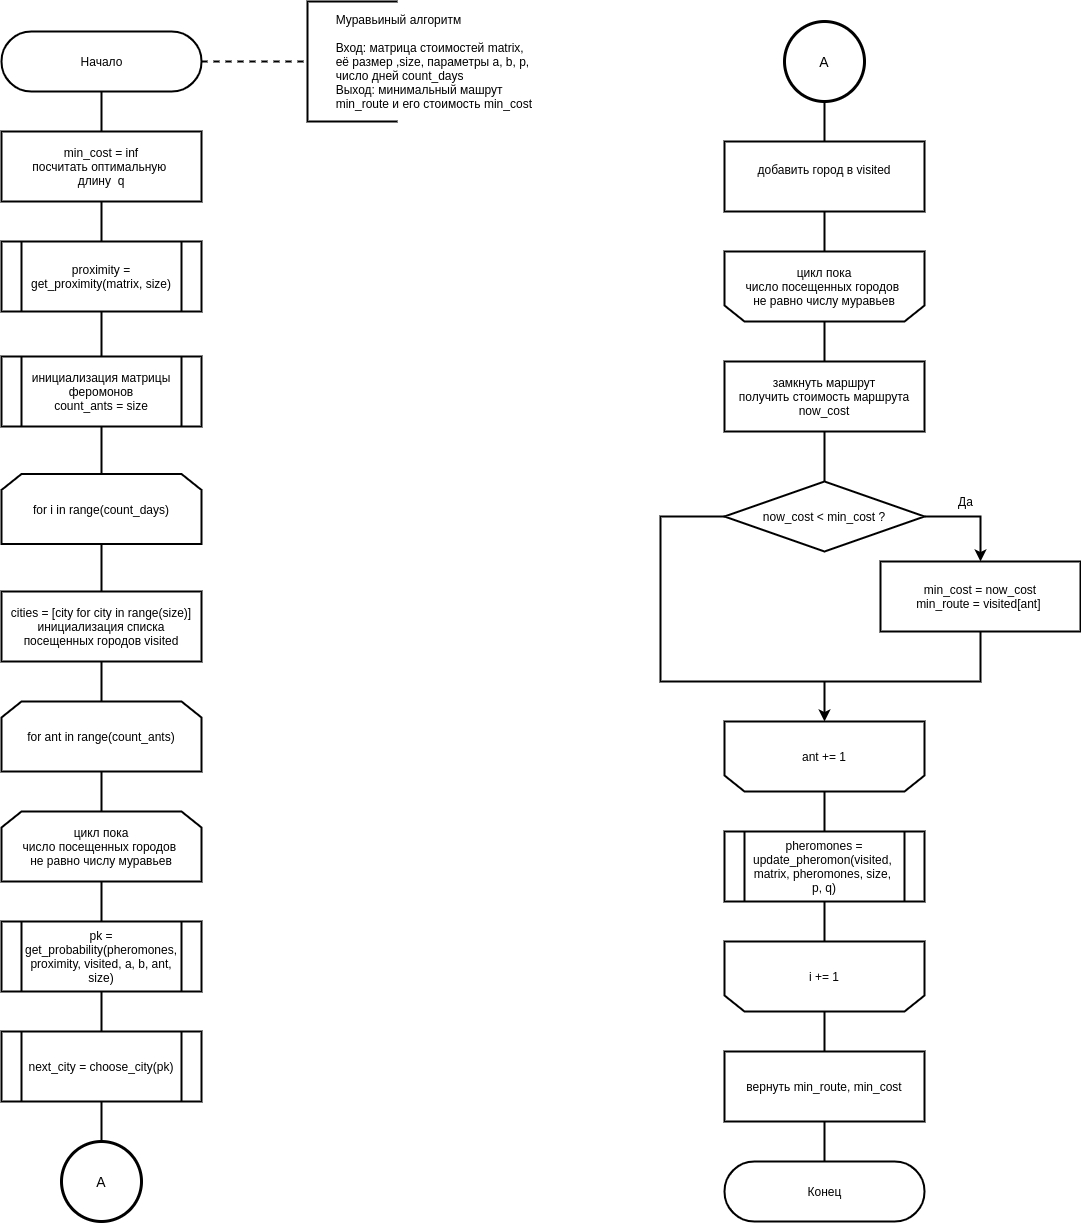
\includegraphics[scale=0.4]{images/ant.png}
	\caption{Муравьиный алгоритм}
	\label{img:ant}
\end{figure}

\begin{figure}[!h]
	\centering
	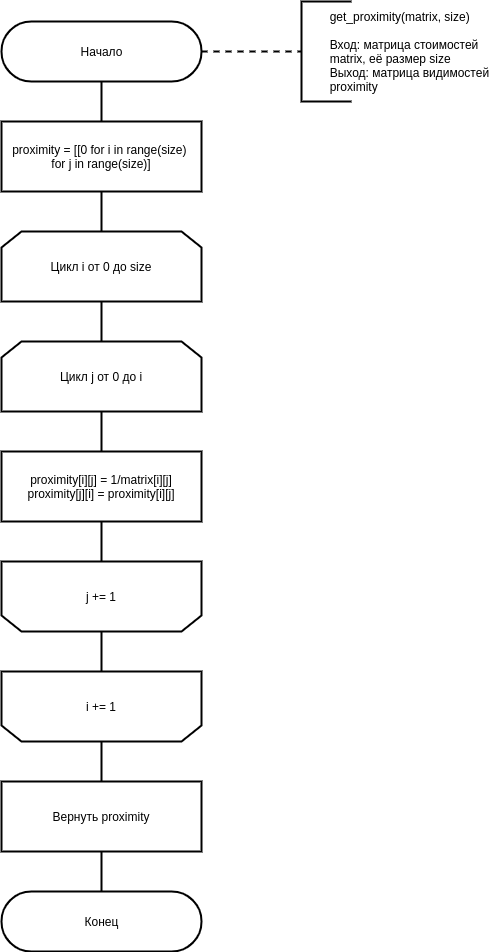
\includegraphics[scale=0.5]{images/proximity.png}
	\caption{Алгоритм вычисления матрицы видимостей}
	\label{img:proximity}
\end{figure}

\begin{figure}[!h]
	\centering
	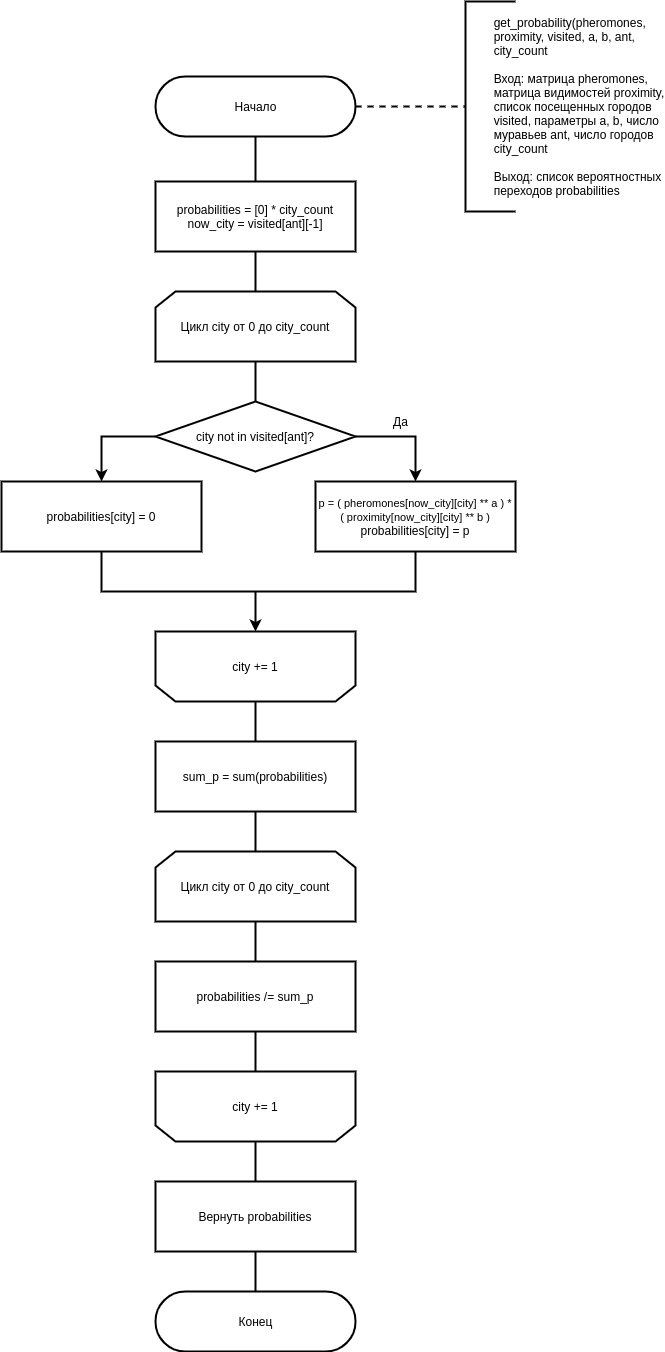
\includegraphics[scale=0.5]{images/probability.png}
	\caption{Алгоритм вычисления списка вероятностных переходов}
	\label{img:probability}
\end{figure}

\begin{figure}[!h]
	\centering
	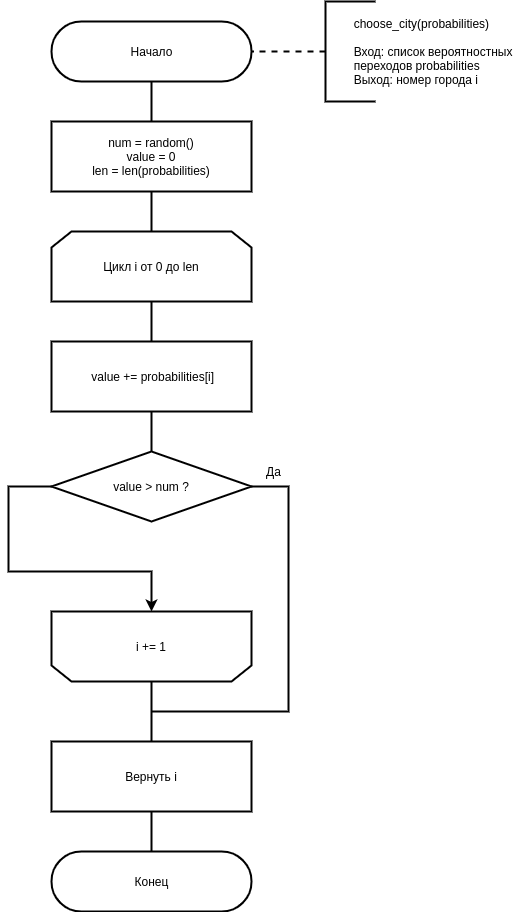
\includegraphics[scale=0.7]{images/choose.png}
	\caption{Алгоритм выбора следующего города случайным образом}
	\label{img:choose}
\end{figure}

\begin{figure}[!h]
	\centering
	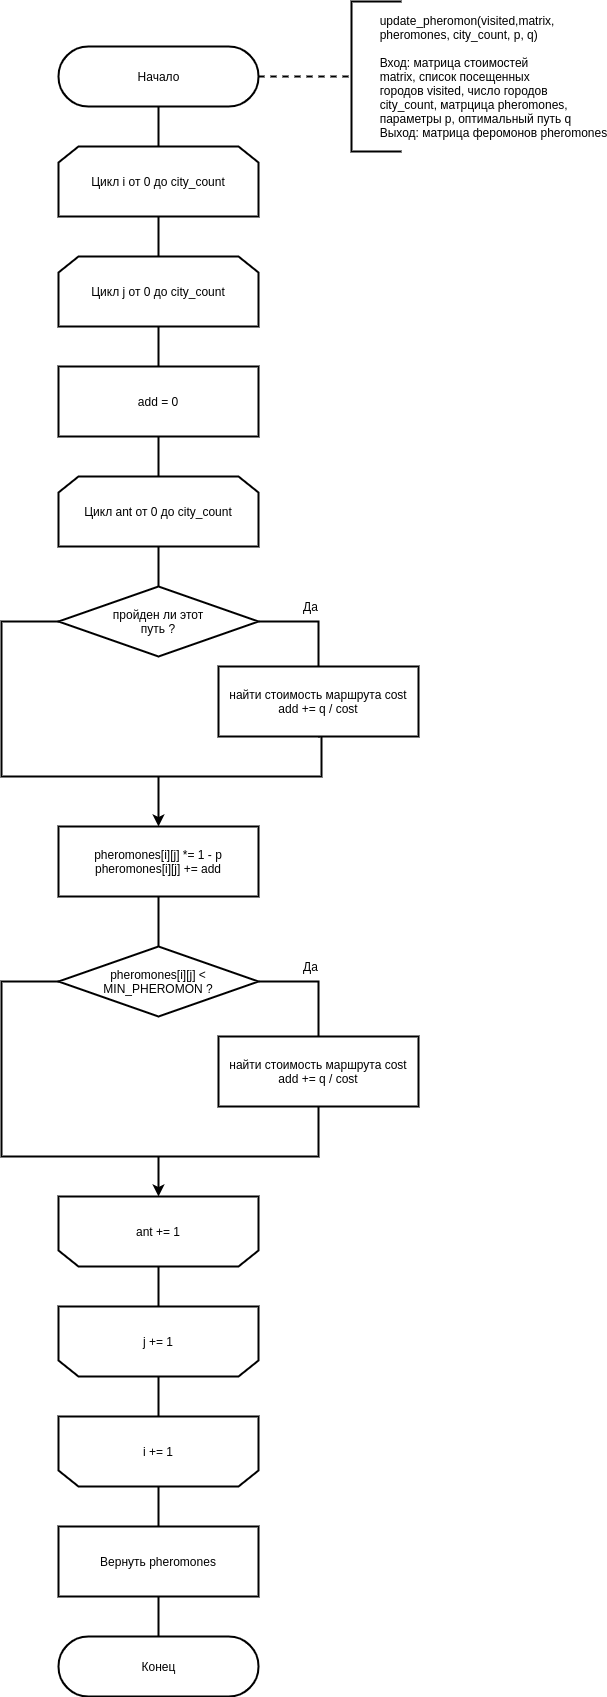
\includegraphics[scale=0.4]{images/update.png}
	\caption{Алгоритм обновления феромона}
	\label{img:update}
\end{figure}
